\documentclass[english,serif,mathserif,usenames,dvipsnames]{beamer}
\usetheme[formal]{s3it}

\usepackage[T1]{fontenc}
\usepackage[utf8]{inputenc}
\usepackage{babel}

%% This is optional: it adds a few commands and environment we
%% regularly use in our slide sets
\usepackage{s3it}

\begin{document}

%% Optional Argument in [Brackets]: Short Title for Footline
\title[Why a Cloud]{Why to build a Cloud}
\subtitle{}
\author{Antonio Messina \texttt{<antonio.messina@uzh.ch>}\\Cloud
  Architect}
\institute{University of Zurich, \sssit}
\date{2 December 2015}
% \titlegraphic{\begin{figure}[ht]\hfill\includegraphics[height=.4\textheight]{SC}
%   \end{figure}
% }

%% Makes the title slide
  \maketitle

\begin{frame}
  {Who are we}

  \sssit is a central service of the University of Zurich.

\+
  We provide solutions for researcher's data analysis usecase:
  \begin{itemize}
  \item Usecase analysis
  \item Solution enginneering and implementaion
  \item tools to run large scale data alaysis and to automate the infrastructure provisioning:
    \begin{itemize}
    \item \href{http://gc3pie.readthedocs.org/en/latest/}{GC3Pie}
    \item \href{http://gc3-uzh-ch.github.io/elasticluster/}{Elasticluster}
    \end{itemize}
  \item Development to implement large-scale data analysis solutions
  \item and the infrastructure where to run it.
  \end{itemize}

\end{frame}

\begin{frame}
  {Researcher's FAQ}

  \begin{itemize}
  \item How can I run this data analysis on 1000 cores since on my
    laptop is too slow? {\scriptsize(btw, I need to submit for
      publication by end of this month)} \+

  \item Where can I put this 100TB of data that I need to analyze and
    share with my colleagues?
    {\scriptsize(did I tell you I have a deadline end of this month?)}
    \+

  \item How can I automate all of this? Can you do it for me? BTW: I
    only know Matlab.
    \+

  \item Do I need to adapt my application to run on your system? Can
    you do it for me?
  \end{itemize}
\end{frame}


\begin{frame}
  {Researchers care about speed}

\only<1>{but what is speed?}

\only<2->{
    \begin{figure}[ht]
    \centering
      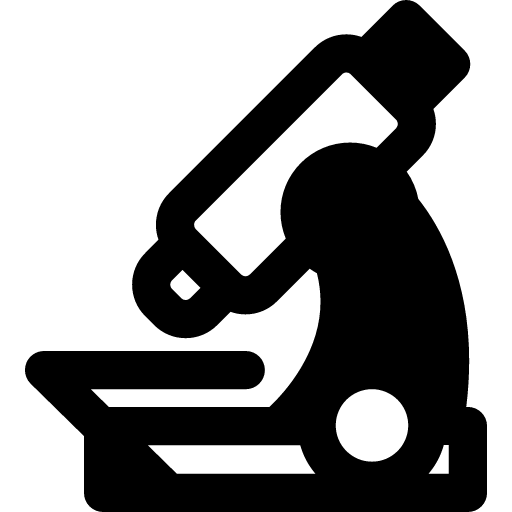
\includegraphics[width=0.2\textwidth]{science27.png}
      \hfill
      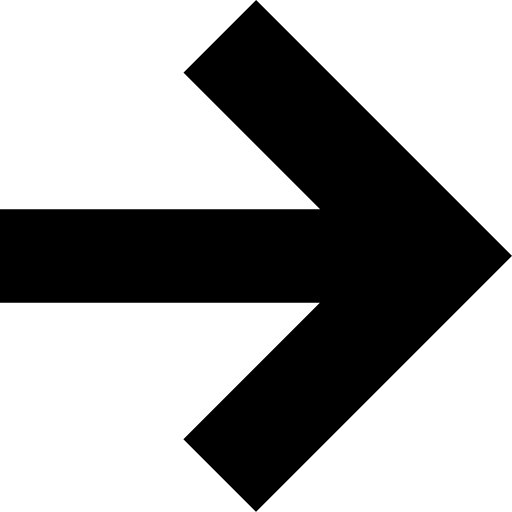
\includegraphics[width=0.2\textwidth]{right208.png}
      \hfill
      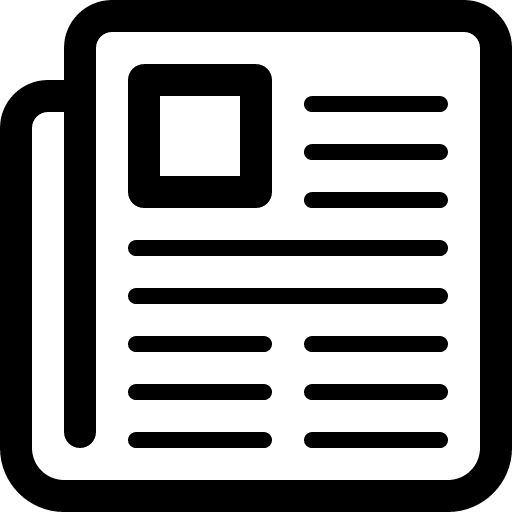
\includegraphics[width=0.2\textwidth]{news29.png}
      \\
      \+
      speed is \textit{\textbf{time to solution}}
  \end{figure}

\begin{itemize}
  \item actual computational time can be a small part
  \item not providing an infrastructure where the researcher can run
    means \textit{no research}
  \item learning curve of adapting an application can be a blocking factor
  \end{itemize}
}
\end{frame}


\begin{frame}
  {What is a cloud?}

  \begin{quotation}
    An infrastructure to provide users with the most flexible way to
    allocate computational power and storage space.
  \end{quotation}
  \+

  \begin{itemize}
  \item \textbf{self-provision} of resources when needed
  \item \textbf{customization} of the infrastructure to the use case
  \item \textbf{automation} of the provisioning of the infrastructure
    \emph{programmatically} (via RESTful APIs)
  \item \textbf{scalability} of the infrastructure
  \item \textbf{Highly Available} infrastructure
  \end{itemize}
  
\end{frame}

\begin{frame}
  {Services a cloud can offer (1/2)}

  \begin{itemize}
  \item \textbf{Compute}: start a VM somewhere\+
  \item \textbf{Block Storage}: create a block device and attach it to
    your VMs\+
  \item \textbf{Object Storage}: a infinite, distributed, highly
    available storage accessible via HTTP (with ACLs)\+
  \item \textbf{Autoscaling}: the ability of automatically spawn or
    destroy VMs based on triggers\+
  \item \textbf{Network}: ability to create complex network
    configurations in the cloud, possibly integrated cloud resources
    with your own network
  % \item Network File system: an elastic POSIX network filesystem that
  %   scales on demand
  % \item Relational databases: create and manage a scalable relational
  %   database
  % \item NoSQL databases: create and manage a scalable NoSQL database
  % \item MessageQueue systems
  \end{itemize}
\end{frame}

\begin{frame}
  {Services a cloud can offer (2/2)}

  \begin{itemize}
  % \item \textbf{Compute}: start a VM somewhere
  % \item \textbf{Block Storage}: create a block device and attach it to
  %   your VMs
  % \item \textbf{Object Storage}: a infinite, distributed, highly
  %   available storage accessible via HTTP (with ACLs)
  % \item \textbf{Autoscaling}: the ability of automatically spawn or
  %   destroy VMs based on triggers
  % \item \textbf{Network}: ability to create complex network
  %   configurations in the cloud, possibly integrated cloud resources
  %   with your own network
  \item Network File system: an elastic POSIX network filesystem that
    scales on demand\+
  \item Relational databases: create and manage a scalable relational
    database\+
  \item NoSQL databases: create and manage a scalable NoSQL database\+
  \item MessageQueue systems\+
  \end{itemize}
\end{frame}

\begin{frame}
  {OpenStack services that we will use}

  \begin{itemize}
  \item \textbf{Horizon}: the web interface
  \+\item \textbf{Nova}: the compute service
  \+\item \textbf{Neutron}: the network service
  \+\item \textbf{Glance}: the image service
  \+\item \textbf{Cinder}: the block storage service
  \+
\end{itemize}
\end{frame}

\end{document}

%%% Local Variables:
%%% mode: latex
%%% TeX-master: t
%%% End:
